
\let\negmedspace\undefined
\let\negthickspace\undefined
\documentclass[journal]{IEEEtran}
\usepackage[a5paper, margin=10mm, onecolumn]{geometry}
%\usepackage{lmodern} % Ensure lmodern is loaded for pdflatex
\usepackage{tfrupee} % Include tfrupee package

\setlength{\headheight}{1cm} % Set the height of the header box
\setlength{\headsep}{0mm}     % Set the distance between the header box and the top of the text

\usepackage{gvv-book}
\usepackage{gvv}
\usepackage{cite}
\usepackage{amsmath,amssymb,amsfonts,amsthm}
\usepackage{algorithmic}
\usepackage{graphicx}
\usepackage{textcomp}
\usepackage{xcolor}
\usepackage{txfonts}
\usepackage{listings}
\usepackage{enumitem}
\usepackage{mathtools}
\usepackage{gensymb}
\usepackage{comment}
\usepackage[breaklinks=true]{hyperref}
\usepackage{tkz-euclide} 
\usepackage{listings}
% \usepackage{gvv}                                        
\def\inputGnumericTable{}                                 
\usepackage[latin1]{inputenc}                                
\usepackage{color}                                            
\usepackage{array}                                            
\usepackage{longtable}                                       
\usepackage{calc}                                             
\usepackage{multirow}                                         
\usepackage{hhline}                                           
\usepackage{ifthen}                                           
\usepackage{lscape}
\usepackage{circuitikz}
\tikzstyle{block} = [rectangle, draw, fill=blue!20, 
    text width=4em, text centered, rounded corners, minimum height=3em]
\tikzstyle{sum} = [draw, fill=blue!10, circle, minimum size=1cm, node distance=1.5cm]
\tikzstyle{input} = [coordinate]
\tikzstyle{output} = [coordinate]


\begin{document}

\bibliographystyle{IEEEtran}
\vspace{3cm}

\title{2.10.42}
\author{EE25BTECH11012 - BEERAM MADHURI}
\maketitle
% \newpage
% \bigskip
{\let\newpage\relax\maketitle}

\renewcommand{\thefigure}{\theenumi}
\renewcommand{\thetable}{\theenumi}
\setlength{\intextsep}{10pt} % Space between text and floats


\numberwithin{equation}{enumi}
\numberwithin{figure}{enumi}
\renewcommand{\thetable}{\theenumi}
% The following content is generated based on the provided image.

\textbf{Question}:\\
If $\mathbf{a}, \mathbf{b}$ and $\mathbf{c}$ are unit coplanar vectors, then the scalar triple product
\[\begin{bmatrix}2\mathbf{a} - \mathbf{b} & 2\mathbf{b} - \mathbf{c} & 2\mathbf{c} - \mathbf{a}\end{bmatrix} =\]\\
\textbf{Solution}:\\
\begin{align}
B = (2\mathbf{a} - \mathbf{b} \quad 2\mathbf{b} - \mathbf{c} \quad 2\mathbf{c} - \mathbf{a}) = (\mathbf{a} \quad \mathbf{b} \quad \mathbf{c})\begin{pmatrix}2 & 0 & -1 \\-1 & 2 & 0 \\0 & -1 & 2\end{pmatrix}
\end{align}

Since $\mathbf{a}$, $\mathbf{b}$, $\mathbf{c}$ are coplanar,
\begin{align}
\begin{vmatrix}\mathbf{a} & \mathbf{b} & \mathbf{c}\end{vmatrix} = 0
\end{align}
\begin{align}
    \begin{vmatrix}2\mathbf{a} - \mathbf{b} & 2\mathbf{b} - \mathbf{c} & 2\mathbf{c} - \mathbf{a}\end{vmatrix} = \begin{vmatrix}\mathbf{a} & \mathbf{b} & \mathbf{c}\end{vmatrix} \begin{vmatrix}2 & 0 & -1 \\-1 & 2 & 0 \\0 & -1 & 2\end{vmatrix} =0
\end{align}

Hence, the value of \begin{bmatrix}2\mathbf{a} - \mathbf{b} & 2\mathbf{b} - \mathbf{c} & 2\mathbf{c} - \mathbf{a}\end{bmatrix} is $0$.\\

\[\text {Proof of } \begin{bmatrix} a & b & c \end{bmatrix} \text{ is singular:}\]
Given $\mathbf{a}$,$\mathbf{b}$,$\mathbf{c}$ are coplanar\\
plane equation of the plane through  $\mathbf{a}$,$\mathbf{b}$,$\mathbf{c}$ be 
\begin{align}
\mathbf{n}^\top \vec{r} = 0
\end{align}
where $\mathbf{n}$ is normal to plane
\begin{align}
\mathbf{n}^\top \Vec{a} &= 0 \\ 
\mathbf{n}^\top \vec{b} &= 0 \\
\mathbf{n}^\top \vec{c} &= 0
\end{align}
let $M = \begin{bmatrix} a & b & c \end{bmatrix}$
\begin{align}
\mathbf{n}^\top M = 0^\top
\end{align}
For a homogeneous linear system
\begin{align}
\mathbf{n}^\top M = 0^\top, \quad \mathbf{n} \neq 0
\end{align}
$M$ must be singular.

\[\therefore \begin{bmatrix} a & b & c \end{bmatrix} \text{ is singular}\]
Hence proved.\\

\begin{figure}[H]
    \centering
    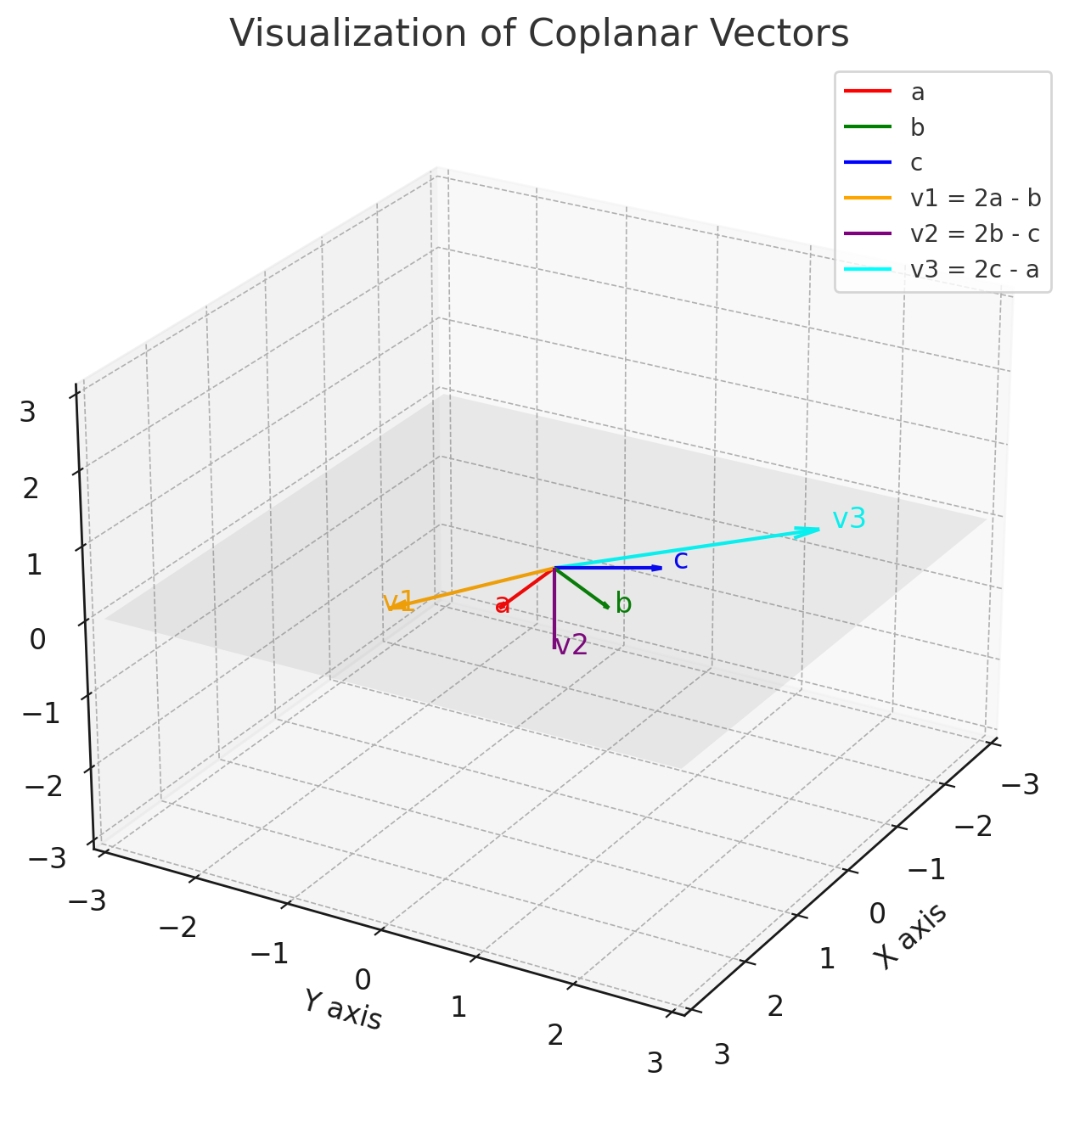
\includegraphics[width=0.75\columnwidth]{figs/graph-1.png}
    \caption{Plot}
    \label{fig:placeholder}
\end{figure}

\end{document}